\documentclass{anstrans}
%%%%%%%%%%%%%%%%%%%%%%%%%%%%%%%%%%%
\title{%
The Nuclear Forensics Problem and Statistical Methods: \\
Evaluating the Nuclear Fuel Cycle with Machine Learning
}
\author{Arrielle C. Opotowsky, Paul P.H. Wilson}

\institute{
Computational Nuclear Engineering Research Group \\
University of Wisconsin at Madison
}

\email{opotowsky@wisc.edu \and paulwilson@wisc.edu}

% Optional disclaimer: remove this command to hide
% \disclaimer{Notice: }

%%%% packages and definitions (optional)
\usepackage{graphicx} % allows inclusion of graphics
\usepackage{booktabs} % nice rules (thick lines) for tables
\usepackage{microtype} % improves typography for PDF

\newcommand{\SN}{S$_N$}
\renewcommand{\vec}[1]{\bm{#1}} %vector is bold italic
\newcommand{\vd}{\bm{\cdot}} % slightly bold vector dot
\newcommand{\grad}{\vec{\nabla}} % gradient
\newcommand{\ud}{\mathop{}\!\mathrm{d}} % upright derivative symbol

\begin{document}
%%%%%%%%%%%%%%%%%%%%%%%%%%%%%%%%%%%%%%%%%%%%%%%%%%%%%%%%%%%%%%%%%%%%%%%%%%%%%%%%
\section{Introduction}

In the event of a nuclear incident, such as the retrieval of stolen nuclear
material or the detonation of a dirty bomb, it is necessary to learn as much as
possible about the source of the materials in a timely manner. To characterize
the materials, both radiological methods (e.g., gamma spectroscopy) and
ionization methods (e.g., mass spectroscopy) are used to determine isotopic
ratios, chemical compounds, or trace elements. Although each category has a
multitude of techniques within it, the main tradeoff is between time/cost and
amount of information gained. 

The results of these analytic techniques are then compared against existing
databases to determine the origin of the nuclear material(s). These databases
are highly multidimensional, and furthermore, are rife with missing data
entries and inconsistent uncertainties. Direct comparison between measurement
results and a database therefore may not yield accurate results. Fortunately,
machine learning algorithms can be explored to create a model from a database
to "fill between the lines".  Additionally, having a machine-learned model may
overcome the above challenges of multidimensionality, missing data, and
irregular uncertainty.

While different machine learning algorithms and parameters will be
investigated, it is first important to determine if statistical methods can
overcome the inherent database deficiencies. Thus, this paper focuses on
probing the amount of information required to obtain realistic results.  This
can be best understood as the analgous real-world scenario.  Although mass
spectroscopy techniques provide extremely accurate isotopic information, they
are time-consuming and more expensice. And although gamma spectroscopy can give
extremely fast results cheaply, it only measures certain radiological signals
and is influenced by many environmental (or storage) factors. In the simulation
and machine learning paradigm, we need to determine what exactly is needed to
train a machine-learned model. Can the algorithm overcome the deficiencies of
gamma detection and still provide useful results? Or does it need more
information, e.g., exact isotopics?

Thus, ultimately, the goal is to answer the question \textit{How does the
ability to determine forensic-relevant spent nuclear fuel attributes degrade as
less information is available?}. But first, we must establish some baseline
expectations and algorithms to use. This work is based off previous work on the
subject (cite Dayman), and expands upon it by also evaluating a more advanced
machine learning algorithm: neural nets. Below is a more in depth discussion of
nuclear forensics and how machine learning can contribute to this research
area. After that, an experimental design is outlined. Lastly, the results are
presented and discussed. 

%%%%%%%%%%%%%%%%%%%%%%%%%%%%%%%%%%%%%%%%%%%%%%%%%%%%%%%%%%%%%%%%%%%%%%%%%%%%%%%%
\section{Background and Theory}

\subsection{Nuclear Forensics}

Nuclear forensics is the analysis and interpretation to determine the history
of nuclear material, whether that be intercepted spent nuclear fuel, uranium
ore concentrate, or the debris from an exploded nuclear device. Technical
nuclear forensics focuses on the characterization and interpretation of those
results. This, in combination with intelligence data, aids in material
attribution, which is the overall goal of nuclear forensics.  

(Something on goal to get as much info as possible within 24 h of interception
or device detonation). 

Nuclear Forensics Workflow Although this focuses on Some materials of special
interest: SNF and reprocessed MOX.  For SNF, measure material, use isotope
content and/or isotope ratios to determine things like reactor type, fuel type
and enrichment at beginning of irradiation, cooling time, burnup. For
reprocessed MOX, ??. 

After the material characteristics are measured, they are matched in a
forensics database that includes some or all this information for
pre-existing/pre-measured SNF/MOX. These databases are kept by individual
countries, and a given database will have widely varying uncertainty depending
where the material was measured as well as missing data in some fields.
Therefore, matching can be difficult.

(Classification, Characterization, Interpretation (Analysis), Reconstruction
(Attribution) - from the New Nuclear Forensics book) (Char methods to get
isotopic ratios or use S/ML, Interp examples)

To accomplish this, (we want to see if) it is possible to limit material
measurements to rapid-result nondestructive analysis, such as gamma ray
spectroscopy. Gamma spec gives less information at a higher uncertainty than
the near perfect results of some destructive mass spec techniques, like TIMS.
Additionally, within gamma spec techniques (field vs lab), uncertainties can
also vary.

\subsection{Machine Learning}

Given imperfect data with varying amounts of uncertainty as well as the
required comparison to imperfect databases, many have begun considering
artificial intelligence approaches to nuclear forensics problems, such as
implementing searching algorithms for database comparison and machine learning
for determining spent fuel characteristics (cite all). A variety of statistical
and machine learning tools have been used to both classify spent fuel (reactor
type, fuel type) and predict values such as burnup, initial enrichment, or
cooling time (regression).

Add some real ML background here
\begin{subequations} \label{eqs:fullTransport}
\begin{multline} \label{eq:fullTransportVol}
  \vec{\Omega}\vd \grad \psi(\vec{x}, \vec{\Omega})
  + \sigma(\vec{x}) \psi (\vec{x}, \vec{\Omega})
\\ =
  \frac{\sigma_s(\vec{x})}{4\pi} \int_{4\pi} \psi(\vec{x},\vec{\Omega}')
  \ud\Omega' + \frac{q(\vec{x})}{4\pi}
  \equiv \frac{1}{4\pi} Q(\vec{x}) \,,
\end{multline}
inside $\vec{x} \in V$, $\vec{\Omega} \in 4\pi$, with an incident boundary
condition
\begin{equation} \label{eq:fullTransportBndy}
  \psi(\vec{x}, \vec{\Omega}) = \psi^b(\vec{x}, \vec{\Omega}) \,,
 \quad \vec{x} \in \partial V, \ \vec{\Omega} \vd \vec{n} < 0\,.
\end{equation}
\end{subequations}

%%%%%%%%%%%%%%%%%%%%%%%%%%%%%%%%%%%%%%%%%%%%%%%%%%%%%%%%%%%%%%%%%%%%%%%%%%%%%%%%
\section{Experimental Design}

Talk about Dayman paper and how I'm extending that, to include neural nets
first and to eval mucking up the training data second.

\subsection{Algorithms Used}

Preprocessing, kNN, ridge, neural net - these are all discussed above, but can
talk deets + parameters here

\subsection{Validation of Each Algorithm}

Classification Training Error: Predetermined test set for training error,
perhaps can make a learning curve (maybe not until there is a variable
train/test set for cross validation)

Classification and Regression Error Confidence: Confidence intervals on error
(helps understand true error versus just the sample error), Test set must be >
30 instances, Can easily calculate N\% confidence interval.

Generalizability should be evaluated (learning more about this with cs760
project)

\subsection{Comparing Algorithms}

Options for comparison of algorithms: Comparing classification of 2 classes on
same ROC plot with multiple ML systems, Scatter plots, Pairwise t-tests

%%%%%%%%%%%%%%%%%%%%%%%%%%%%%%%%%%%%%%%%%%%%%%%%%%%%%%%%%%%%%%%%%%%%%%%%%%%%%%%%
\section{Results and Analysis}
The results were interesting, so interesting in fact that we have decided to
present them here.

%%%%%%%%%%%%%%%%%%%%%%%%%%%%%%%%%%%%%%%%%%%%%%%%%%%%%%%%%%%%%%%%%%%%%%%%%%%%%%%%
\subsection{Subsection Goes Here}
The user must manually capitalize initial letters of a subsection heading.

For those who like equations in their papers, \LaTeX\ is a good choice. Here is
an equation for the Marshak diffusion boundary condition:
\begin{equation} \label{eq:marshak}
  4 J^- = \phi + 2 D \vec{n} \vd \grad \phi \,.
\end{equation}
If we so choose, we can effortlessly reference the equation later.

Another paragraph starts with Eq.~\eqref{eq:marshak} and sets $J^-$ to zero, a
vacuum boundary condition:
\begin{equation*}
  0 = \phi + \frac{2}{3} \frac{1}{\sigma} \vec{n} \vd \grad \phi \,.
\end{equation*}
The extrapolation distance is $2/3$. A more detailed asymptotic analysis yields
an extrapolation distance of about $0.71045$.

Figure~\ref{fig:voltage} shows how a plot might conceivably look in your
document. Always place figures after they are referenced so as not to throw
off the reader. You can use symbols and different line styles to help
differentiate your results, especially if they are printed in black and white.
Note how Fig.~\ref{fig:voltage} uses dashed lines \verb|--| for the exact
solution, solid lines \verb|-| for the new method's solutions, and dotted lines
\verb|:| for existing inaccurate methods.
\begin{figure}[ht] % replace 't' with 'b' to force it to be on the bottom
  \centering
  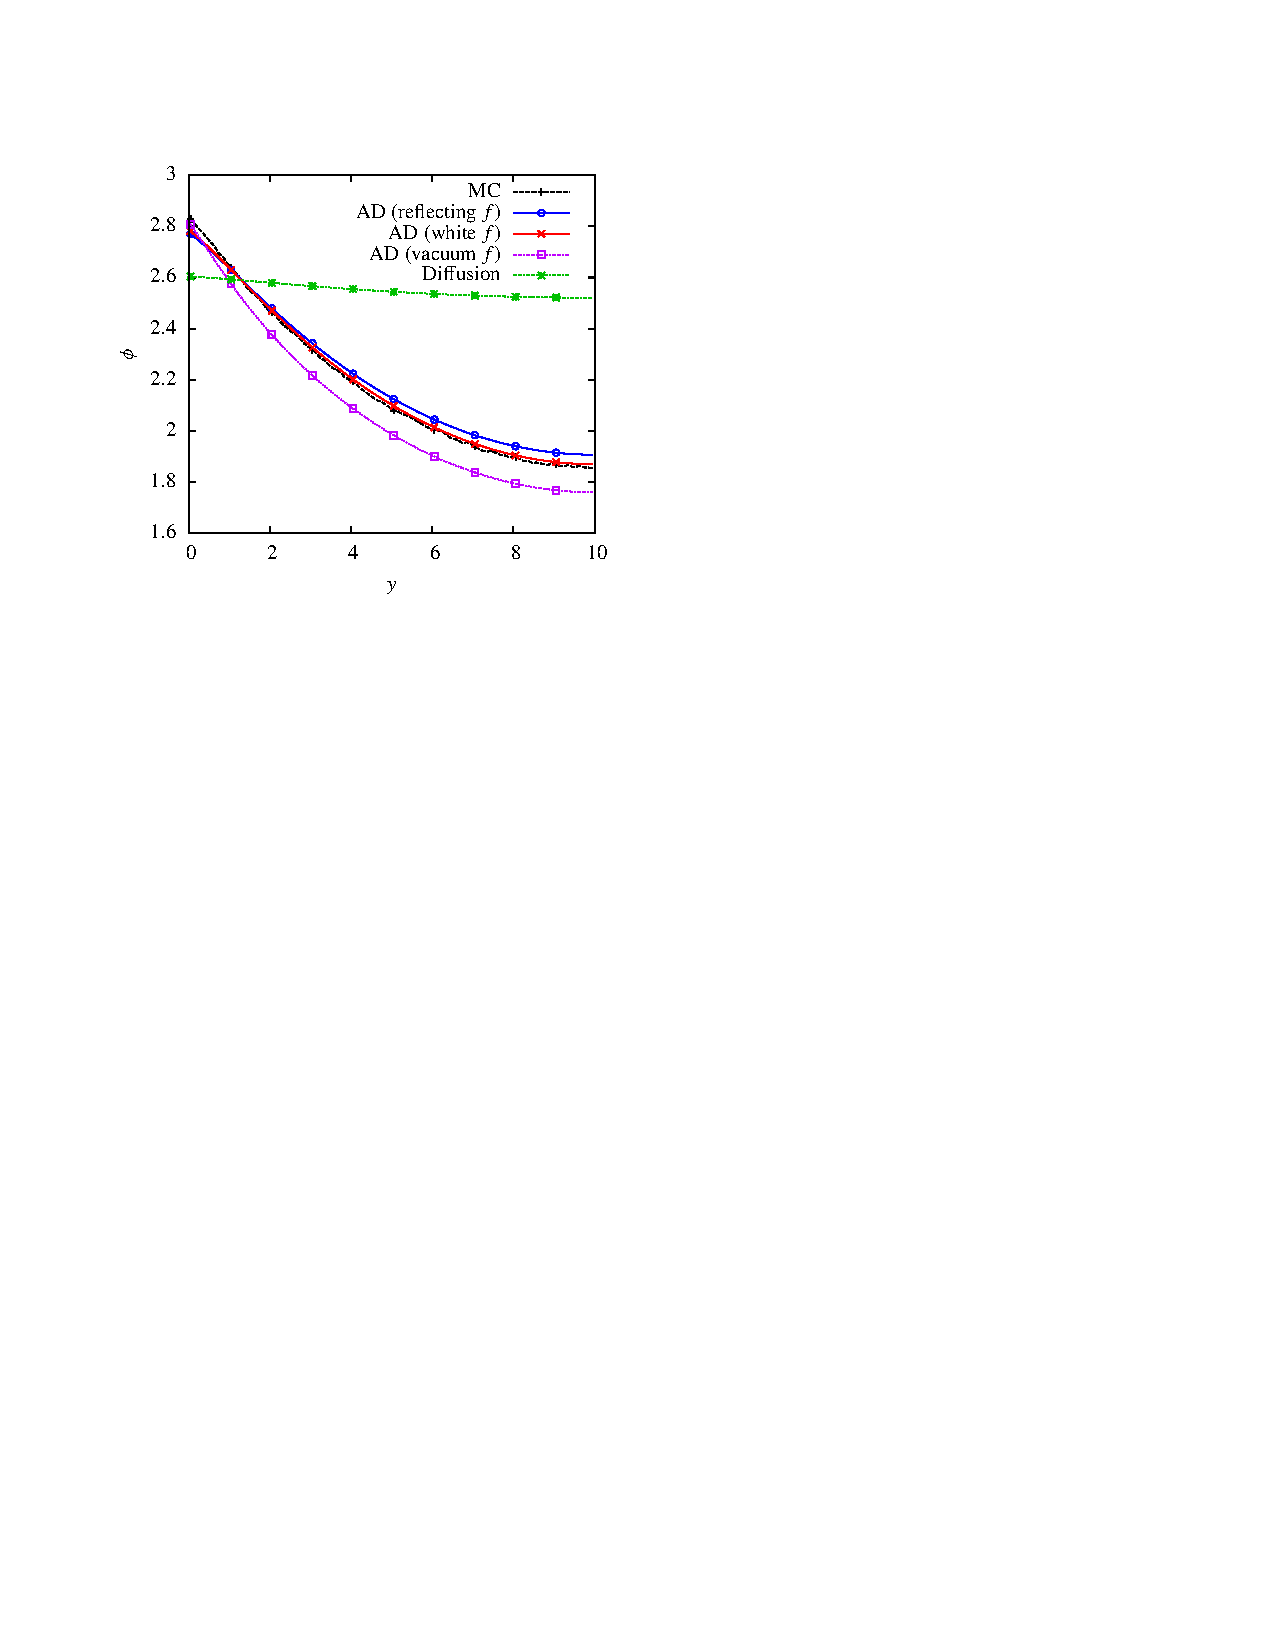
\includegraphics{example_figure}
  \caption{Captions are flush with the left.}
  \label{fig:voltage}
\end{figure}

Later on, we can include a table, even one that spans two columns such as
Table~\ref{tab:widetable}.
%%%%%%%%%%%%%%%%%%%%%%%%%%%%%%%%%%%%%%%%
\begin{table*}[htb]
  \centering
\begin{tabular}{llllllllll}\toprule
      & $\phi_T(0)$      & $\phi_T(10)$      & $\phi_T(20)$      &
      $\phi_D(0)$      & $\phi_D(10)$      & $\phi_D(20)$      & $\rho$      &
      $\varepsilon$      & $N_\text{it}$
\\ \midrule
$c=0.999$  & 0.9038 & 20.63 & 31.24 & 0.9087 & 20.63 & 31.23 & 0.2192 & $10^{-7}$ & 15
\\
$c=0.990$  & 0.3675 & 13.04 & 24.7 & 0.3696 & 13.04 & 24.69 & 0.2184 & $10^{-7}$ & 15
\\
$c=0.900$  & 0.009909 & 4.776 & 17.64 & 0.009984 & 4.786 & 17.63 & 0.2118 & $10^{-7}$ & 14
\\
$c=0.500$  & $6.069\times 10^{-5}$ & 2.212 & 15.53 & 6.213$\times 10^{-5}$ & 2.239 & 15.53 & 0.2068 & $10^{-7}$ & 13
\\
\bottomrule
\end{tabular}
  \caption{This is an example of a really wide table which might not normally
  fit in the document.}
  \label{tab:widetable}
\end{table*}
%%%%%%%%%%%%%%%%%%%%%%%%%%%%%%%%%%%%%%%%
Notice how the table reference uses a Roman numeral
for its numbering scheme, whereas the figure reference uses an Arabic numeral.
For one-column tables, use the \verb|table| environment; two-column tables use
\verb|table*|. The same applies to figures.

%%%%%%%%%%%%%%%%%%%%%%%%%%%%%%%%%%%%%%%%%%%%%%%%%%%%%%%%%%%%%%%%%%%%%%%%%%%%%%%%
\subsection{Another Subsection}
Excessive sectioning in a three-page document is discouraged, but here are more
subsections to demonstrate compliance with the ANS formatting guidelines.

\subsubsection{Third-level Heading}
This subsubsection shows compliance with the ANS-specified standard. This level
of heading should be used rarely.

\subsubsection{Another Such Heading}
And, if you really think you need a third-level heading, you should make sure
that your subsection needs at least two of them.

%%%%%%%%%%%%%%%%%%%%%%%%%%%%%%%%%%%%%%%%%%%%%%%%%%%%%%%%%%%%%%%%%%%%%%%%%%%%%%%%
\section{Conclusions}

The included ANS style file and this clear example file are a panacea for
the hours of headache that invariably results from formatting a document in
Microsoft Word.

%%%%%%%%%%%%%%%%%%%%%%%%%%%%%%%%%%%%%%%%%%%%%%%%%%%%%%%%%%%%%%%%%%%%%%%%%%%%%%%%
\appendix
\section{Appendix}

Numbering in the appendix is different:
\begin{equation} \label{eq:appendix}
  2 + 2 = 5\,.
\end{equation}
and another equation:
\begin{equation} \label{eq:appendix2}
  a + b = c\,.
\end{equation}

%%%%%%%%%%%%%%%%%%%%%%%%%%%%%%%%%%%%%%%%%%%%%%%%%%%%%%%%%%%%%%%%%%%%%%%%%%%%%%%%
\section{Acknowledgments}
This material is based upon work supported a Department of Energy Nuclear
Energy University Programs Graduate Fellowship.

%%%%%%%%%%%%%%%%%%%%%%%%%%%%%%%%%%%%%%%%%%%%%%%%%%%%%%%%%%%%%%%%%%%%%%%%%%%%%%%%
\bibliographystyle{ans}
\bibliography{bibliography}
\end{document}

